\documentclass[conference]{IEEEtran}
\usepackage{fancyhdr}

\usepackage{cite}
\usepackage{amsmath,amssymb,amsfonts}
\usepackage{url}
%\usepackage{algorithmic}
\usepackage{graphicx}
%\usepackage{textcomp}
\usepackage{listings}
\usepackage[caption=false]{subfig}
\usepackage{xcolor}
\usepackage{flushend} % Equalize columns on last page.


\def\BibTeX{{\rm B\kern-.05em{\sc i\kern-.025em b}\kern-.08em
    T\kern-.1667em\lower.7ex\hbox{E}\kern-.125emX}}

\newsavebox{\histogrambox}
\newsavebox{\genhistogrambox}
\newsavebox{\goldseqhisto}
\newsavebox{\fullyatomichisto}
\newsavebox{\fullyparhisto}
\newsavebox{\chunkedhisto}
\newsavebox{\sortscanhisto}
\newsavebox{\multicoophisto}
\newsavebox{\RTXoneGlb}
\newsavebox{\RTXoneLoc}
\newsavebox{\RTXsixtyLoc}
\newsavebox{\RTXsixtyGlb}
\newsavebox{\RTXcub}

% Define Language
\lstdefinelanguage{futhark}
{
  % list of keywords
  morekeywords={
    do,
    else,
    for,
    fun,
    if,
    in,
    include,
    let,
    loop,
    struct,
    then,
    type,
    val,
    while,
    with,
    module,
    where,
    sort,
    multired
  },
  sensitive=true, % keywords are not case-sensitive
  morecomment=[l]{--}, % l is for line comment
  morecomment=[s]{\{-}{-\}}, % s is for start and end delimiter
%  otherkeywords={>,<,=,<=,>=,!,*,/,-,+,|,&,||,&&,==,=>},
  morestring=[b]", % defines that strings are enclosed in double quotes
  literate={\\}{\fn}{1} {->}{$\rightarrow$}{1} {<-}{$\leftarrow$}{1},
}

\lstdefinelanguage{corefuthark}
{
  % list of keywords
  morekeywords={
    do,
    else,
    for,
    fun,
    if,
    in,
    include,
    let,
    loop,
    struct,
    then,
    type,
    val,
    while,
    with,
    module,
    where,
  },
  sensitive=true, % keywords are not case-sensitive
  literate={\\}{\fn}{1} {->}{$\rightarrow$}{1} {<-}{$\leftarrow$}{1},
  moredelim=**[is][\color{red}]{@}{@},
  morecomment=[l]{--}, % l is for line comment
  morecomment=[s]{\{-}{-\}}, % s is for start and end delimiter
%  otherkeywords={>,<,=,<=,>=,!,*,/,-,+,|,&,||,&&,==,=>},
  morestring=[b]" % defines that strings are enclosed in double quotes
}

% Define Colors
\usepackage{xcolor}
\definecolor{eclipseBlue}{RGB}{42,0.0,255}
\definecolor{eclipseGreen}{RGB}{63,127,95}
\definecolor{eclipsePurple}{RGB}{127,0,85}

\newcommand{\fop}[1]{\mbox{\ttfamily\color{eclipseBlue}#1}}
\newcommand{\fw}[1]{\mbox{\ttfamily\bfseries\color{eclipsePurple}#1}}

% Set Language
\lstset{
  language={futhark},
  basicstyle=\small\ttfamily, % Global Code Style
  extendedchars=true, % Allows 256 instead of 128 ASCII characters
  tabsize=2, % number of spaces indented when discovering a tab
  columns=fixed, % make all characters equal width
  keepspaces=true, % does not ignore spaces to fit width, convert tabs to spaces
  showstringspaces=false, % lets spaces in strings appear as real spaces
  numbers=none, % do not show line numbers at the left
  numberstyle=\footnotesize\ttfamily, % style of the line numbers
  commentstyle=\itshape\color{eclipseGreen}, % style of comments
  keywordstyle=\bfseries, % style of keywords
  stringstyle=\color{eclipseBlue}, % style of strings
  emph=[1] {
    atomic,
    false,
    filter,
    forall,
    forseq,
    iota,
    map,
    map2,
    map4,
    partition,
    rearrange,
    reduce,
    reduce_comm,
    redomap,
    scanomap,
    replicate,
    reshape,
    rotate,
    shape,
    scan,
    split,
    true,
    unzip,
    scatter,
    zip,
    stream_seq,
    stream_red,
    stream_map,
    stream_par,
    size,
    manifest,
    local,
    kernel,
    stream_group,
    red_by_index,
    sort,
    transpose
  },
  emphstyle=\ttfamily\bfseries,
  moredelim=**[is][\color{red}]{@}{@},
}

\newcommand{\Dom}{{\rm Dom}}
\newcommand{\ov}[1]{\overline{#1}}
\newcommand{\nseq}[2]{\overline{#1}^{(#2)}}
\newcommand{\seq}[1]{\overline{#1}}
\newcommand{\LR}[1]{\langle #1\rangle}
\newcommand{\hsp}{\hspace{5mm}}
\newcommand{\kt}[1]{\textsf{#1}}
\newcommand{\kw}[1]{\mbox{\texttt{\bfseries{#1}}}}
\newcommand{\id}[1]{\mbox{\it{#1}}}
\newcommand{\M}[2]{\LR{#1\in #2}}
\newcommand{\Mv}[2]{\LR{\seq{#1}\in\seq{#2}}}
\newcommand{\Mvv}[4]{\LR{\seq{#1}\,\seq{#2}\in\seq{#3}\,\seq{#4}}}
\newcommand{\Do}{\kw{do}}
\newcommand{\For}{\kw{for}}
\newcommand{\Map}{\kw{map}}
\newcommand{\fn}{\ensuremath{\lambda}}
\newcommand{\Fn}[3]{\fn#2:~#1~\rightarrow #3}
\newcommand{\FnU}[2]{\fn#1~\rightarrow #2}
\newcommand{\Reduce}{\kw{reduce}}
\newcommand{\Reshape}{\kw{reshape}}
\newcommand{\Redomap}{\kw{redomap}}
\newcommand{\Scanomap}{\kw{scanomap}}
\newcommand{\Scan}{\kw{scan}}
\newcommand{\Transpose}{\kw{transpose}}
\newcommand{\Let}[3]{\kw{let}~#1~\mbox{\texttt{=}}~#2~\kw{in}~#3}
\newcommand{\Lett}[3]{\!\begin{array}[t]{l}\kw{let}~#1~\mbox{\texttt{=}}~#2 \\\kw{in}~#3 \end{array}}
\newcommand{\If}[3]{\kw{if}~#1~\kw{then}~#2~\kw{else}~#3}
\newcommand{\Iff}[5]{\begin{array}[t]{l}\kw{if}~#1~\kw{then}~ #2\\\kw{else}~\kw{if}~#3~\kw{then} ~#4 \\\kw{else}~#5\end{array}}
\newcommand{\Loop}[5]{\kw{loop}~#1~\texttt{=}~#2~\kw{for}~#3<#4~\kw{do}~#5}
\newcommand{\Loopp}[5]{\begin{array}[t]{l}\kw{loop}~#1~\texttt{=}~#2~\kw{for}~#3<#4~\kw{do}\\\hsp #5\end{array}}
\newcommand{\vd}{\vdash}
\newcommand{\Rearrange}{\kw{rearrange}}
\newcommand{\Replicate}{\kw{replicate}}
\newcommand{\Par}[1]{\mathtt{(}#1\mathtt{)}}
\newcommand{\SqPar}[1]{\mathtt{[}#1\mathtt{]}}
\newcommand{\Set}[1]{\{#1\}}
\newcommand{\StreamMap}{\kw{stream\_map}}
\newcommand{\StreamRed}{\kw{stream\_red}}
\newcommand{\StreamPar}{\kw{stream\_par}}
\newcommand{\StreamSeq}{\kw{stream\_seq}}
\newcommand{\StreamGroup}{\kw{stream\_group}}
\newcommand{\Segmap}{\kw{segmap}}
\newcommand{\Segred}{\kw{segred}}
\newcommand{\Segscan}{\kw{segscan}}
\providecommand{\G}{}
\renewcommand{\G}[1]{G#1}
\newcommand{\sembox}[1]{\hfill \normalfont \mbox{\fbox{\(#1\)}}}
\newcommand{\sempart}[2]{\textrm{\textit{#1 \sembox{#2}}}}

\newcommand{\fract}[3]{\vspace{2mm}\mbox{$\frac{\begin{array}{c} #2 \end{array}}{\begin{array}{c} #3 \end{array}}$}~[\mbox{\textsc{#1}}]}
\newcommand{\onepart}[1]{\noindent\hfill#1\hfill\mbox{~}}
\newcommand{\twopart}[2]{\noindent\hfill#1\hfill#2\hfill\mbox{~}}
\newcommand{\threepart}[3]{\noindent\hfill#1\hfill#2\hfill#3\hfill\mbox{~}}

%%% Local Variables:
%%% mode: latex
%%% TeX-master: "icfp18"
%%% End:


\newcommand\ToDo[1]{\textcolor{red}{#1}}
\newcommand\lmad{\textsc{lmad~}}
\newcommand\lmads{\textsc{lmad}s~}

\begin{document}

\title{Memory Optimizations in an Array Language %Functional
\thanks{Identify applicable funding agency here. If none, delete this.}
}

\author{
  \IEEEauthorblockN{Philip Munksgaard}
  \IEEEauthorblockA{\textit{University of Copenhagen} \\
    Copenhagen, Denmark}
  \and
  \IEEEauthorblockN{Troels Henriksen}
  \IEEEauthorblockA{\textit{University of Copenhagen} \\
    Copenhagen, Denmark}
  \and
  \IEEEauthorblockN{Ponnuswamy Sadayappan}
  \IEEEauthorblockA{\textit{University of Utah}\\
    Salt Lake City, USA}
  \and
  \IEEEauthorblockN{Cosmin Oancea}
  \IEEEauthorblockA{\textit{University of Copenhagen} \\
    Copenhagen, Denmark}
}


\maketitle
%\thispagestyle{fancy}
%\lhead{}
%\rhead{}
%\chead{}
%\lfoot{\footnotesize{SC20, November 9-19, 2020, Is Everywhere We Are\newline
%    978-1-7281-9998-6/20/\$31.00 \copyright 2020 IEEE}}
%\rfoot{}
%\cfoot{}
%\renewcommand{\headrulewidth}{0pt}
%\renewcommand{\footrulewidth}{0pt}

\begin{abstract}
to be filled in
\end{abstract}

\begin{IEEEkeywords}
GPU, parallelism, functional programming, optimizing compiler
\end{IEEEkeywords}

\section{Introduction}
\label{sec:introduction}

\begin{itemize}
% Paragraph stating that in an imperative context the user
% is expected to optimize memory usage and access patterns.
\item In the context of imperative programming, the programming
        model allows (and even encourages) the user to equate
        memory buffers with arrays, and to perform various
        memory-related optimizations, aiming for example:
        (1) at decreasing the memory footprint by (re)using the same
            memory buffer to hold (at different times) semantically
            different arrays, and
        (2) at optimizing locality and copying overheads by
            inlining together reads and writes to/from the same array,
            inside a parallel construct.

% Paragraph presenting the shortcomming of the "imperative"
% solutions: results in code with complex indices,
% hinders code maintinability, and opportunities for
% compiler optimizations. Essentially, parallel semantics
% is not verifyable.
\item One the one hand, such memory optimizations enable efficient
       implementations that utilize well the memory system. On the
       other hand, the downsides are that the resulted code
        (1) is less maintinable, typically using complex (non-affine)
            indexing (e.g., flattened indices) and more prone to bugs,
        (2) might hinder further compiler optimizations. For example
            many of the challenging cases pertaining automatic
            parallelization were the result of the compiler having to
            reverse-engineer users' memory optimizations--see the
            considerable amount of work in the context of Polaris and
            SUIF compilers and polyhedral compilation. A classic example
            is that the application of loop-skewing and block tiling
            results in un-analyzable non-affine code.
    In particular, in such context it is infeasible to enforce
    a correct-by-construction parallel semantics, which is verifiable
    at language level (e.g., by means of simple typeching-like mechanisms).

% Present at high level the functional context
\item In the functional (data-parallel) context, all available
        parallelism is expected to be explicitly expressed by means
        of second-order operators---that take arrays (and a function/operator)
        as parameters and produce new arrays---such as map, reduce, scan
        (prefix sum). As such, parallelism is
        ``correct-by-construction'' because cross-iteration
        dependencies cannot appear when the read and write accesses
        are performed on different arrays. The safety of parallelization
        is thus verifiable by type-checking mechanisms, even when
        a restricted form of in-place updates are
        allowed~\cite{futhark-pldi}.
        In addition, functional programming models support various
        operations that change the layout of the arrays (but does not
        modify its elements), such as slicing, rotation, rearanging
        array dimensions (e.g., transposition).   In principle,
        such operations can be supported in constant time, e.g.,
        by representing arrays as index functions and aggressively
        fusing them~\cite{data-par-haskell, svensson2011obsidian}.

\item The downside of such approaches are (1) suboptimal memory
        footprint---because each operation may create a new array,
        and (2) copying overhead.
        The latter is necessary in order to enforce the
        ``correct-by-construction'' guarantee. Figure~\ref{fig:nw-hl}
        demonstrates this neccessity for the NW problem ...

% Short summary of what is this work about
\item This work addresses the
\end{itemize}

\begin{figure}
\centering
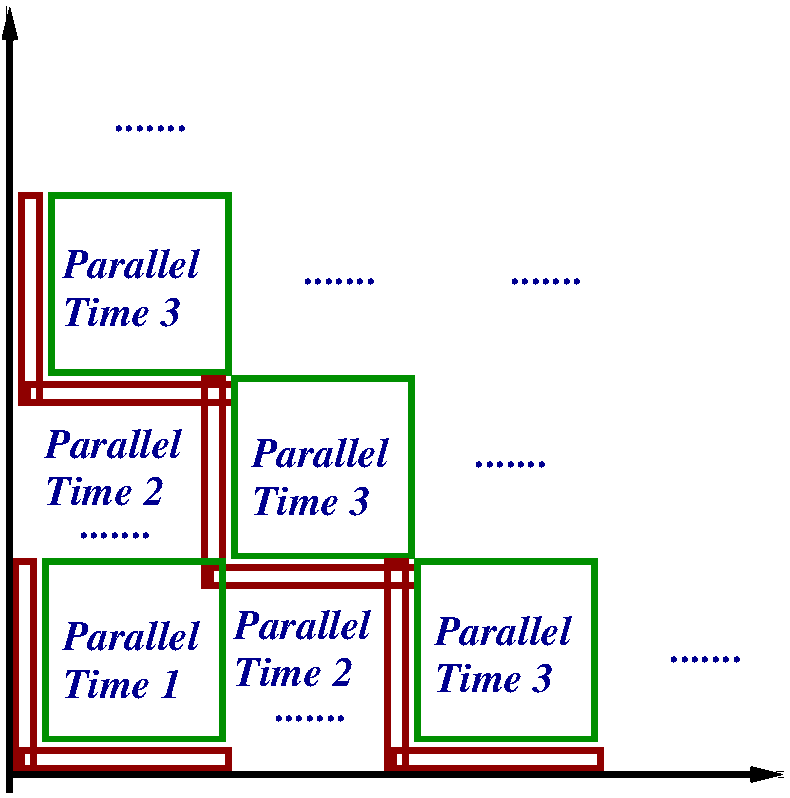
\includegraphics[width=0.25\textwidth]{figs/nw-hl}
\caption{NW parallel access patterns}
\label{fig:nw-hl}
\end{figure}


\section{Preliminaries}
\label{sec-prelims}

This section is supposed to introduce by example,
in corresponding subsections, at least:
\begin{itemize}
\item[1] the idea that arrays can be represented as
         index functions, e.g., used to achieve fusion
         in functional languages;
\item[2] the definition and use of \lmads in imperative
         analyses aimed at automatic parallelization
         of loop-based code, including the procedure
         for aggregating \lmads across loop indices.
\item[3] the semantics of the source (and target)
         language used in this paper.
\end{itemize}

\subsection{Arrays as Index Functions}
\label{subsec:ixfun-intro}

\ToDo{Troels, are you taking a shot at this?}

\subsection{Linear Memory Access Descriptor (LMAD)}
\label{subsec:lmad-intro}


An \lmad essentially defines a set of (linearized)
uni-dimensional points that have a regular, quasi-affine structure:
%
\begin{scriptsize}
\begin{equation}
\tau + \{\ov{(n:s)}^q\} \ \ \equiv \ \ \{ \ \tau + i_1 \cdot s_1  + \ldots + \ i_{q}\cdot s_{q} \ \ \ | \ \ \ 0 \leq i_k < n_k, \ k = 1\ldots q\}\label{def-lmad}
\end{equation}
\end{scriptsize}
%
A $q$-dimensional \lmad consists of an offset $\tau$ and a
sequence of $q$ tuples $(n_i,s_i)$ that represent for each dimension $i$:
\begin{itemize}
\item[$n_i$:] its number of points, referred to as {\em cardinality}, and
\item[$s_i$:] the (linearized) distance between two consecutive points
              on that dimension, referred to as {\em stride}.
\end{itemize}

Complex inter-procedural analyses have used \lmads as a basic block
for building summaries of memory references across large loop nests,
for example in analysis aimed at proving loop parallelism based on
set equations written in terms of the read-only, write-first and
read-write sets.

\lmads power resides in that they represent by definition a
set of flat indices but they ``form'' dimensions according to how
the underlying memory is used (rather than to how the array was declared).
%
For example, \lmads allow analysis
\begin{itemize}
\item  to be performed on flat indices, which are not affine,
\item to be extended across procedure boundaries where
     arrays are permitted to change shape (e.g., in Fortran77).
\end{itemize}

%label={fig:loop-nest-orig},caption={Original Loop}
\begin{lstlisting}[mathescape,basicstyle=\ttfamily\scriptsize]
-- assuming positive M, N, k
do i = 0 $\ldots$ M-1        -- $W = \cup_{i=0}^{M-1} W_{i} = t + \{(M:M),(N:k)\}$
  do j = 0 $\ldots$ N-1      -- $W_i = \cup_{j=0}^{N-1} W_{i,j} = t + i*M + \{(N:k)\}$
    A[t + i*M + j*k] = ... -- $W_{i,j} = t + i*M + j*k \ + \ \{\}$
\end{lstlisting}
The example below demonstrates how the write access to {\tt A}
is aggregated across the two nested loops of indices {\tt i} and
{\tt j}. Initially, inside the two loops, the \lmad $W_{i,j}$
is the point $\{t + i*M + j*k\}$



\subsection{Language}
\label{subsec:lang-intro}

\ToDo{Troels, are you taking a shot at this?}

\section{Bird's Eye View Example}
\label{sec:nw-hl}

\section{LMAD-based Representation of Memory}
\label{sec:mem-rep}

\subsection{LMADs as Index Functions}
\label{subsec:lmad-ixfn}

\subsection{Mapping Change-of-Layout Transformations}
\label{subsec:lmad-ops}

\subsection{Anti-Unification over Control Flow}
\label{subsec:lmad-gen}

\section{Array Shortcircuiting Optimization}
\label{sec:arr-shcirc}

\subsection{High-Level Overview}
\label{subsec:shcirc-hl}


\begin{itemize}
\item present the problem statement and the intuition behind our solution, demonstrated on simple examples;

\item establish the notation, e.g., array creation point, coalescing point;

\item present at a high level the four safety conditions necessary for array shortcircuiting to fire:
    \begin{itemize}
    \item the memory of {\tt ys} is already allocated at the creation point of {\tt bs}'s root;
    \item {\tt bs} is lastly used in the ``coalescing statement'' {\tt ys[slc] = bs$^{lu}$};
    \item the index function of {\tt bs} is expressible at the definition point, and the same holds for all arrays aliased with {\tt bs};
    \item index analysis that proves that it is safe to allocate {\tt bs} in the memory space of {\tt ys}
    \end{itemize}

\item based on this, give a road-map of this section, i.e., what issue is discussed in which subsection.

\item Point out that we discuss in a separate subsection special cases, such as loop and if statements, and we discuss in the last subsection our solution to solving LMAD-based equations.
\end{itemize}


\subsection{Treatment of Aliases}
\label{subsec:shcirc-aliases}

\subsection{Loop, If and Map Statements}
\label{subsec:shcirc-aliases}

\subsection{LMAD-Based Index Analysis}
\label{subsec:idx-anl}

\subsection{Solving LMAD Equations}
\label{subsec:lmad-eqs}

\section{Memory Reuse Optimization}
\label{sec:regalloc}

\section{Experimental Evaluation}
\label{sec:exp-eval}

\subsection{Experimental Methodology}
\label{subsec:exp-meth}

\subsection{Study Case NW}
\label{subsec:exp-nw}

\subsection{Study Case LUD}
\label{subsec:exp-lud}

\subsection{Study Case HotSpot}
\label{subsec:exp-hotspot}

\subsection{Bulk Validation}
\label{subsec:bulk-val}

\section{Related Work}
\label{sec:rel-work}

\section{Conclusions}
\label{sec:concl}

\newpage

\bibliographystyle{IEEEtran}
\bibliography{IEEEabrv,sc22-mem.bib}

\end{document}
% end of file template.tex

%%% Local Variables:
%%% mode: latex
%%% TeX-master: t
%%% End:
